\setlength{\parindent}{0pt}
\clearpage

\section{Liveness DFA example}
(Prepared by Jai Arora)
\vspace{0.3cm}

Consider the following example:

\begin{figure}[H]
        \centering
        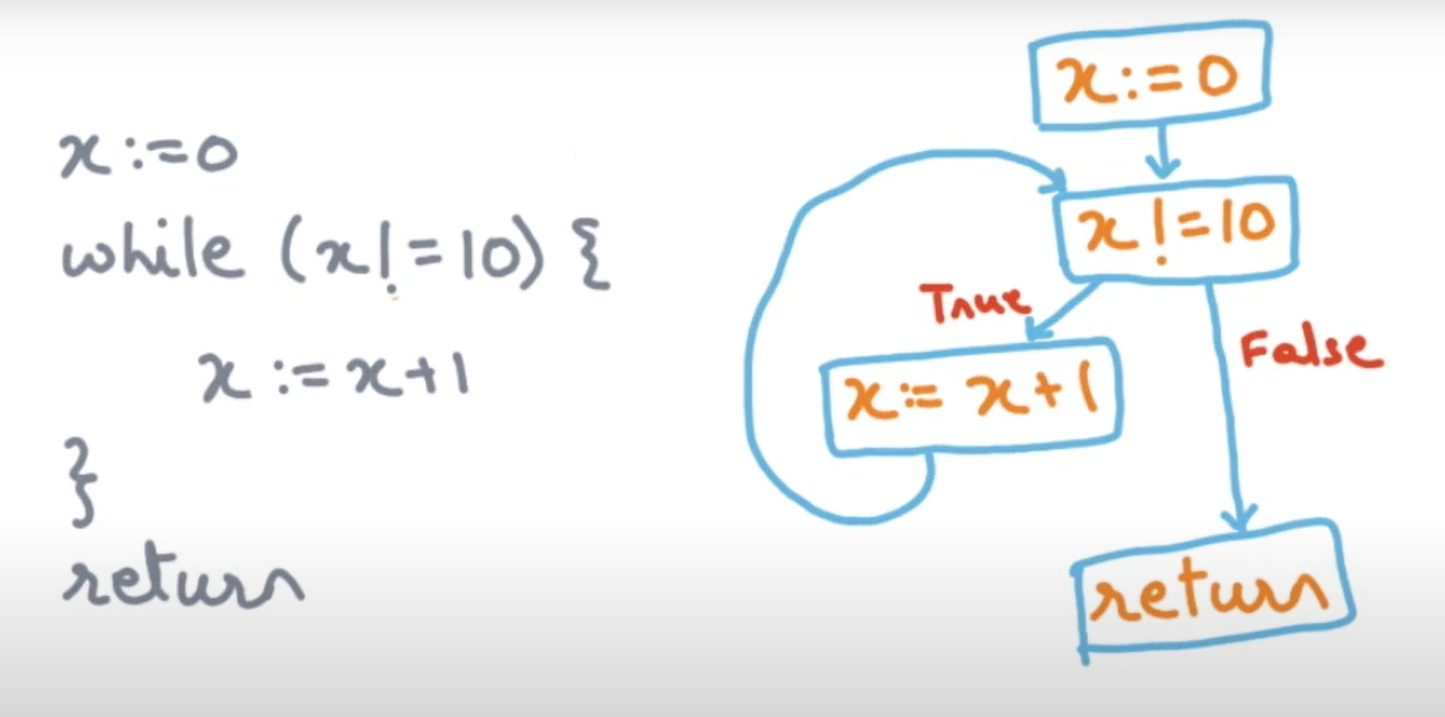
\includegraphics[height=6cm]{images/Module83_1.png}
\end{figure}

The solution for this program using the Liveness DFA rules discussed is follows:
\begin{figure}[H]
        \centering
        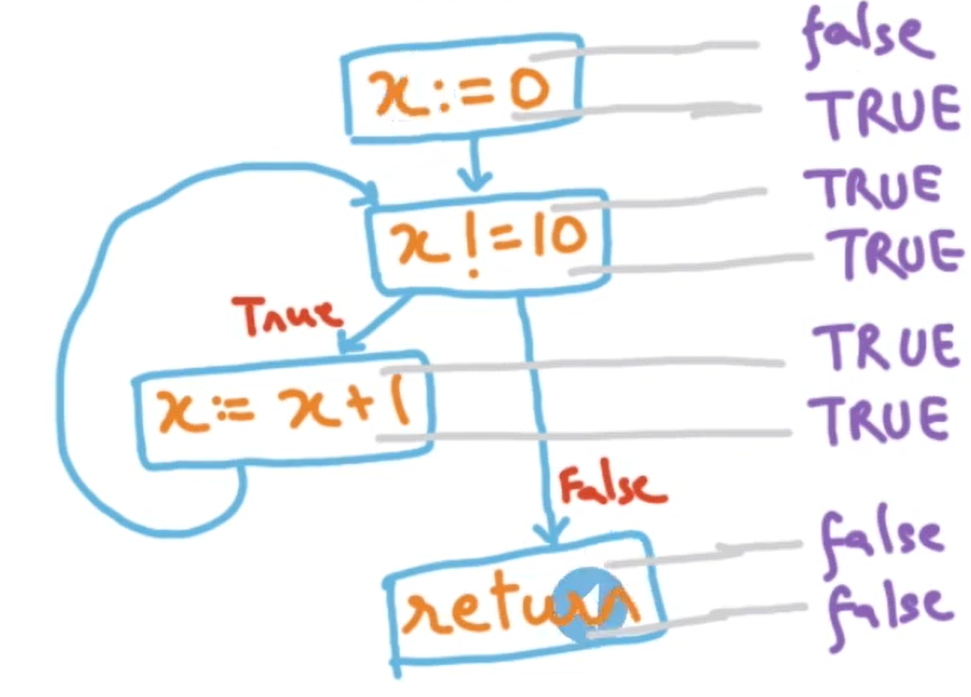
\includegraphics[height=6cm]{images/Module83_2.png}
\end{figure}

The working of this example can be found in \href{https://www.youtube.com/watch?v=dTVq4gnbUYg&list=PLf3ZkSCyj1tf3rPAkOKY5hUzDrDoekAc7&index=83}{this video}.\\

\subsection{Liveness DFA Observations}
\begin{itemize}
    \item Every $L()$ in this analysis can change only once (${\tt false} \rightarrow {\tt true}$). Now this fact guarantees the convergence of the fixed point algorithm.
    \item Worst Case execution time: For a particular variable, all the $L()$ can change only once, and as the number of such values is $2 \times \#$statements, so the worst case execution time is $O(2 \times \#$statements).
    \item Once this analysis is finished, we can use it to identify dead code.
    \item Notice that information flowed in the forward direction (in the direction of the program execution) for constant propagation but flowed in the reverse direction (against the direction of the program execution) for liveness analysis.
    The former types of analyses are called forward dataflow analyses. The latter types of analyses are called backward dataflow analyses
\end{itemize}